\documentclass[11pt,oneside,letterpaper]{article}

% graphicx package, useful for including eps and pdf graphics
\usepackage{graphicx}
\DeclareGraphicsExtensions{.pdf,.png,.jpg}

% basic packages
\usepackage{color}
\usepackage{parskip}
\usepackage{float}

% text layout
\usepackage{geometry}
\geometry{textwidth=15cm} % 15.25cm for single-space, 16.25cm for double-space
\geometry{textheight=22cm} % 22cm for single-space, 22.5cm for double-space

% helps to keep figures from being orphaned on a page by themselves
\renewcommand{\topfraction}{0.85}
\renewcommand{\textfraction}{0.1}

% bold the 'Figure #' in the caption and separate it with a period
% Captions will be left justified
\usepackage[labelfont=bf,labelsep=period,font=small]{caption}

% review layout with double-spacing
%\usepackage{setspace}
%\doublespacing
%\captionsetup{labelfont=bf,labelsep=period,font=doublespacing}

% cite package, to clean up citations in the main text. Do not remove.
\usepackage{cite}
%\renewcommand\citeleft{(}
%\renewcommand\citeright{)}
%\renewcommand\citeform[1]{\textsl{#1}}

% Remove brackets from numbering in list of References
\renewcommand\refname{\large References}
\makeatletter
\renewcommand{\@biblabel}[1]{\quad#1.}
\makeatother

\usepackage{authblk}
\renewcommand\Authands{ \& }
\renewcommand\Authfont{\normalsize \bf}
\renewcommand\Affilfont{\small \normalfont}
\makeatletter
\renewcommand\AB@affilsepx{, \protect\Affilfont}
\makeatother

% notation
\usepackage{amsmath}
\usepackage{amssymb}

% Inline comments by initials
\def\jhc#1{\textcolor{red}{[#1]}}
\definecolor{purple}{rgb}{0.459,0.109,0.538}
\def\tbc#1{\textcolor{purple}{[#1]}}

%%% TITLE %%%
\title{\vspace{1.0cm} \Large \bf
Fitness models provide accurate short-term forecasts of SARS-CoV-2 variant frequency
}
%
\author[1,2,*]{Eslam Abousamra}
\author[1,3,*]{Marlin Figgins}
\author[1,2,4]{Trevor Bedford}

\affil[1]{Vaccine and Infectious Disease Division, Fred Hutchinson Cancer Center, Seattle, WA, USA}
\affil[2]{Department of Epidemiology, University of Washington, Seattle, WA, USA}
\affil[3]{Department of Applied Mathematics, University of Washington, Seattle, WA, USA}
\affil[4]{Howard Hughes Medical Institute, Seattle, WA, USA}
\affil[*]{These authors contributed equally to this work.}


\date{}

\begin{document}

\maketitle

%%% ABSTRACT %%%
\begin{abstract}

Genomic surveillance of pathogen evolution is essential for public health response, treatment strategies, and vaccine development.
In the context of SARS-COV-2, multiple models have been developed including Multinomial Logistic Regression (MLR), Fixed Growth Advantage (FGA), Growth Advantage Random Walk (GARW) and Piantham that use observed variant sequence counts through time to analyze variant dynamics.
These models provide estimates of variant fitness and can be used to forecast changes in variant frequency.
We introduce a framework for evaluating real-time forecasts of variant frequencies, and apply this framework to the evolution of SARS-CoV-2 during 2022 in which multiple new viral variants emerged and rapidly spread through the population.
We compare models across representative countries with different intensities of genomic surveillance.
Retrospective assessment of model accuracy highlights that most models of variant frequency perform well and are able to produce reasonable forecasts.
We find that the simple MLR model provides less than 1\% mean absolute error when forecasting 30 days out for countries with robust genomic surveillence.
We investigate impacts of sequence quantity and quality across countries on forecast accuracy and conduct systematically downsampling to identify that 1000 sequences per week is fully sufficient for accurate short-term forecasts.
We conclude that fitness models represent a useful prognostic tool for short-term evolutionary forecasting.

\end{abstract}

%%% INTRODUCTION %%%
\section*{Introduction}

Mathematical and statistical modeling of infectious diseases plays a key role in predicting the growth of epidemics.
Understanding the trends and characteristics of emerging epidemics can guide public health officials to control their spread \cite{ding_value_2021}.
Epidemiologists face a multitude of challenges in order to \jhc{cut phrases like these} provide accurate and timely predictions of disease spread.
With the increased availability of genomic sequencing, there have been efforts to use sequencing as a tool for investigating the genetic diversity, evolution, and transmission of epidemic-causing pathogens \cite{gire_genomic_2014,zhou_pneumonia_2020}.
More recently, with the upscaling and deluge of sequence data from various testing centers, issues with data arise regarding quantity \jhc{issue is scaling analyses/storage with increasing data. what else?}, near-real-time accessibility, availability, and quality of sequences.
%Integration of these data sources
Data collected from different geographical locations and time-points exhibit varying degrees of missing data, submission delays, and back-filling of disease occurrence which leads to differences in the quantities and availability of sequencing data on different observation dates \cite{crepey_challenges_2022}.
This variability in sequence availability can adversely impact the accuracy and reliability of forecasting efforts using mathematical models \cite{suchard_bayesian_2018}.
Different modeling approaches may have varying levels of sensitivity to imperfections or limitations in the data.
Even when data are complete and accurate, the chosen model may not be suitable for the problem being analyzed, resulting in inability to capture target trends \cite{gelman_bayesian_2013}.
Thereby, it is essential to take these factors, both data-wise and with regard to systematic methodological errors or biases into account when using mathematical models to make predictions, as they can impact the accuracy and reliability of the model's output \cite{crepey_challenges_2022}.


Mathematical models elucidate disease processes and have been sought to assess the risk of and frame the response to emerging pathogens.
Representation of disease spread from genomic sequences can forecast disease occurrence and pathogen frequencies, which refer to the relative abundance or prevalence of specific pathogens within a population, that allows to uncover the inherent characteristics of emerging pathogens and compare potential mechanisms of spread and persistence in the population \cite{metcalf_opportunities_2017}.
%mention importance of forecasting variant frequences and estimating growth advantage
In particular, forecasting variant frequencies allows us to interrogate the impact of mutation accumulation and viral diversity on the spread of and competition between different variants in the population.
The biological selective advantage of specific variants results in increased transmissibility or immune evasion which confers variants' growth advantages in which enable us to make inferences by estimating their variability \cite{tegally_detection_2021}.
The validity and reliability of these mathematical models depend on the quality and quantity of data used for the model \cite{tao_biological_2021}.
With the emergence of novel pathogens, real-time data scarcity represents a real challenge to accurate forecasts and nowcasts, which are short-term forecasts that differ from traditional long-term forecasts, as it leads to increased uncertainty in identifying and forecasting epidemic trends \cite{metcalf_opportunities_2017}. 


%what we actually did (high level)

To investigate how modeling approaches \jhc{Which modeling approaches? Need more background on the models before you describe how you evaluate them.} handle data issues, we developed a framework for evaluating model nowcast and forecast of real-time SARS-CoV-2 variant frequencies, due to their high data availability and diversity, within several countries including (Australia, Brazil, Japan, South Africa, the
United Kingdom, and the United States).
%what is interesting about the framework (key points) comparing various models > applicable to real-time surveillance
To investigate the effectiveness of these different modeling approaches in the context of infectious disease prediction, we implemented the framework utilizing SARS-CoV-2 genomic sequence data and several \jhc{Which} models of frequency change for model comparison and evaluation.
%Specifically, we focused on models of increasing complexity, which were fitted using the evofr (evolutionary forecasting) software package in Python.
%several metrics such as , RMSE, and Sequence log likelihood
To assess the performance of these models, we used mean absolute error (MAE) as a metric to compare the predicted frequencies to a set of known true values (smoothed raw frequency values of SARS-CoV-2 variants \jhc{This parenthetical is a little too detailed for the introduction but is great for the methods}). %what is truth set (Smoothed raw_freq)
This metric allowed us to evaluate the accuracy and reliability of the models and to identify those that were most effective in predicting SARS-CoV-2 circulating variants trends.
We also examined a variety of variables that may contribute to the emergence of errors in these models.
Our aim was to identify the variables that play a role in our ability to forecast variant frequencies.
We explored the role of sequence availability on nowcast and forecast errors through scaling back sequencing efforts for a sample location. 
Through these analyses, we develop a deeper understanding of the factors that contribute to errors in nowcasting and forecasting on genomic surveillance data for pathogens, and ultimately contribute to the ongoing efforts to understand and improve the accuracy of these evolutionary forecasting models.
%What explains our errors
%try to explain the persistent patterns in the errors


%limits of their use-ability

%I use Google Scholar format for citation style with first author, year and first word of title, ala \cite{hadfield2018nextstrain}.


%%% RESULTS %%%
\section*{Results}

%TALKING ABOUT PROCESS FIGURES

\paragraph{Live Forecasting Environment}\

%TODO: What do we mean by live forecasting...
%Due to the ...., sequecnes are submitted ... Basically give a bit of detail to ground reader in what environment we're wroking in
Nowcasting variant frequencies is complicated by the ongoing nature of the data submission process.
\jhc{Can you rewrite the following sentence to summarize the data in Figure 1 that illustrate the effects of variation across countries? The current sentence leaves the reader to figure out what the meaningful results are.}
Figures presented in 1A and 1B offers a visual representation of the live nowcasting environment, illustrating the significance of incorporating observational data in our forecasting models and the variations that exist among countries in terms of the utilization and impact of such data.
The representation emphasizes the variability and back-filling of sequencing data at different observation dates for both the US and Japan. 
%MF:Being specific about the model isn't necessary here and which model can be mentioned in the caption alone. If we're talking about what's going on in Figure 1, I would say that directly and cite it \ref{fig:Figure1}
Utilizing sequencing data for these variants \jhc{Which variants and why?}, we conducted a comparative analysis of the availability of SARS-CoV-2 variants sequences in Japan and the United States \jhc{Why focus on these two countries?} as observed for different observation dates along the period of February 15th to December 1st, 2022 which was chosen due to the its prominent dynamic behavior with multiple clade replacement for SARS-CoV-2 \cite{:ck_markov_covid}  (Figure~\ref{fig:dynamic_forecast_env}A).
Throughout the observation period, the United States had a higher availability of SARS-CoV-2 sequences compared to Japan.
Nonetheless, both countries exhibited variability in sequence availability count for the same dates depending on observation dates. 


% We then evaluated the model performance by analyzing the input sequence data available for Japan and the United States on specific observation dates.
We fit the Growth Advantage Random Walk (GARW) model within our framework at each of these observation dates to demonstrate the nature of the real-time forecasting environment for five different SARS-CoV-2 variants (Omicron 21K, 21L, 21A, 22B, 22C) (Figure \ref{fig:dynamic_forecast_env}.B).
We used these data to predict the frequencies of SARS-CoV-2 variants in these countries, and compared these predictions to 7-day smoothed frequencies of variant occurrence (Figure~\ref{fig:dynamic_forecast_env}B).
However, we observed that the model predictions for Japan were more frequently misestimated compared to United States, this is presented in frequency estimates for clades 22B and 22E (Figure~\ref{fig:dynamic_forecast_env}B).



%MF: In general, we want to be a bit more direct. These are not just the data there are predictions here as well. Really this figure is about a "Live nowcasting environment".
%%% map %%%
\begin{figure}[H]
	\centering
	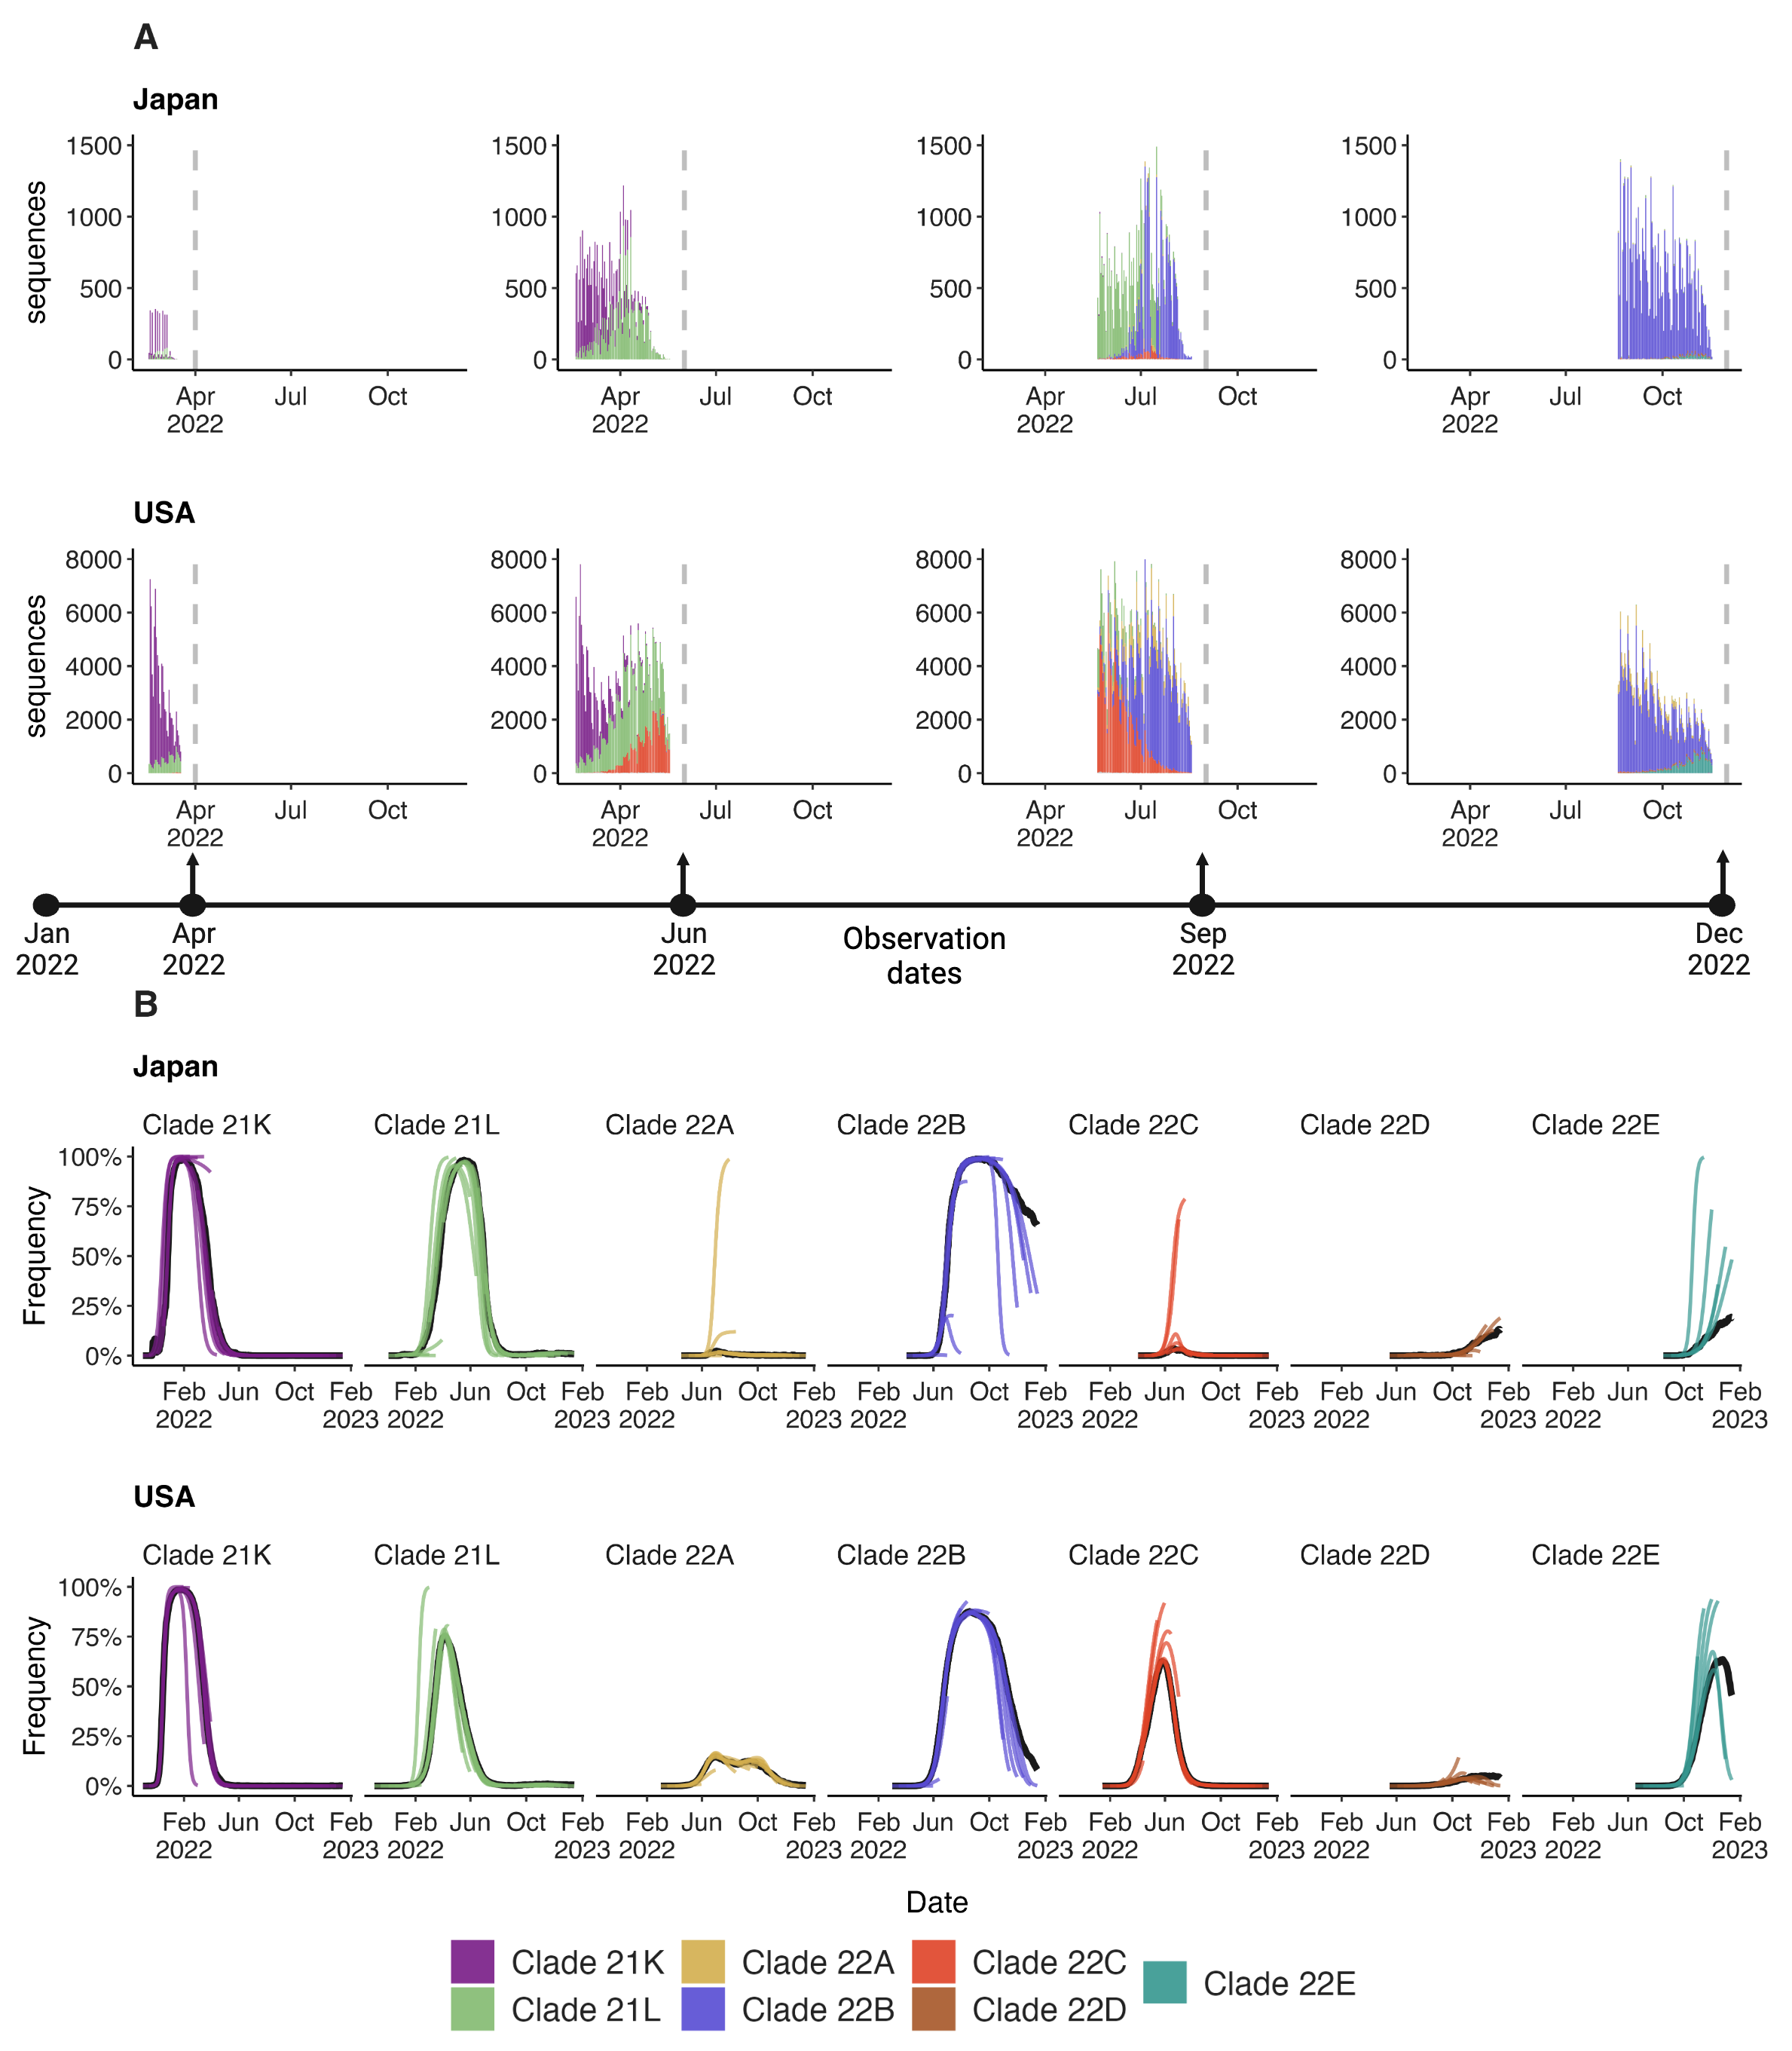
\includegraphics[width=0.8\textwidth=0.01]{figures/Dynamic_est_env.png}
	\caption{\textbf{Representative data and predictions for Japan and USA.}
    Figure 1 represents a schematic of the real-time forecasting environment.
    \jhc{The goal of this figure was to compare Japan and the USA, but the difference in scales on the y-axis between the two countries complicates that comparison. Have you tried plotting both countries on the same scale? Alternately, scaling the number of sequences by the number of cases or people in the country could place the two rows of part A on the same scale.}
	(A) Variant sequence counts from Japan and United States are shown at 3 different observation dates.
	Notice varying sequence availability at different observation dates.
	(B) Frequency nowcasts for variants Nextstrain clades (21K, 21L, 22A, 22B, 22C, 22D, 22E), which depends on the data, vary by observation date. 
	Retrospective smoothed frequency is represented in black, nowcasts are estimated for each clade with the data available at different observation dates. }
	\label{fig:dynamic_forecast_env}
  %MF: Figure filenames and labels we typically want to describe what's in the figure itself since the order is usually subject to change.
\end{figure}


\paragraph{Model Error Comparison}\

We began our model comparison by calculating the difference in days between the date of observation and the date of estimation (lag times) as a means of evaluating the performance of the models per each variant, country, and observation date.
This approach provides a reference for understanding how the models perform as the lag time decreases from the forecast period to the nowcast period, where the lag time approaches zero (the date of observation), specifically from 30 days before the date of observation and 30 days after the date of observation [-30,30].
This method enables us to evaluate the effectiveness of the models as we move closer to and further away from the date of observation.

We applied a total of five models for predicting the frequencies of SARS-CoV-2 variants in six countries representing six continents (Australia, Brazil, Japan, South Africa, the United Kingdom, and the United States).
The first four models are Growth Advantage Random Walk (GARW) \cite{figgins_bedford_freq_dyn}, Fixed Growth Advantage (FGA) \cite{figgins_bedford_freq_dyn}, Multinomial Logistic Regression (MLR), and Piantham \cite{piantham2021estimating}, which are evolutionary forecasting models varying in complexity, refer to methods for more details.
We compare the above 4 models to a naive model to serve as a reference model for comparison \jhc{Need a definition of the naive model here esp. since it is a baseline model.}.
It is a baseline model which uses simple assumptions to make predictions. %todo mention that this model is worse and that is based on a moving average % mentioned in methods

The use of multiple models that range in complexity allows for a comprehensive evaluation of the performance and robustness of different forecasting methods.
In particular, the use of multiple models allows us to examine if more complex models may be better at capturing epidemiological variant patterns.

%Mention which models performed best in each lead (no need to mention numbers)
We used our predictions and used a metric from the framework, specifically mean absolute error (MAE), to assess the relative performance of the models for the six countries (Table~\ref{table:model_comp_table}).
The use of MAE as a metric allows us to quantitatively compare the predictions of different models and determine which model is most accurate in terms of predicting the frequencies of SARS-CoV-2 variants \jhc{Tighten up}.
The model with the lowest mean MAE error for each country is highlighted as it indicates the best performance among all models (Table~\ref{table:model_comp_table}).
There was a range of values \jhc{What was the range?} among the models for different lags.
In this analysis, the GARW model performed the best, on average, for -30 days from the date of estimation.
For 0 and 30 days from the date of estimation, the MLR outperformed, on average, all other models.
For 0 and 30 days, GARW model performed similarly well \jhc{How well? Report the relevant numbers that support your statement}, with the MLR model exhibiting better performance in United Kingdom, Brazil, and Japan, while the GARW model demonstrated better performance in South Africa.
These findings indicate that the GARW model exhibited the best performance \jhc{I was confused to see this conclusion, since the two sentences prior the MLR model outperformed all other models. Then, the more I thought about it, the less I understood how ``best'' is evaluated here. Is the best based on the mean of the MAE across all six countries?}, as measured by mean absolute error (MAE), among the models evaluated, excluding the naive reference model.
In contrast, the Piantham model performed worst on average among the models tested.

\begin{figure}[H]
	\centering
	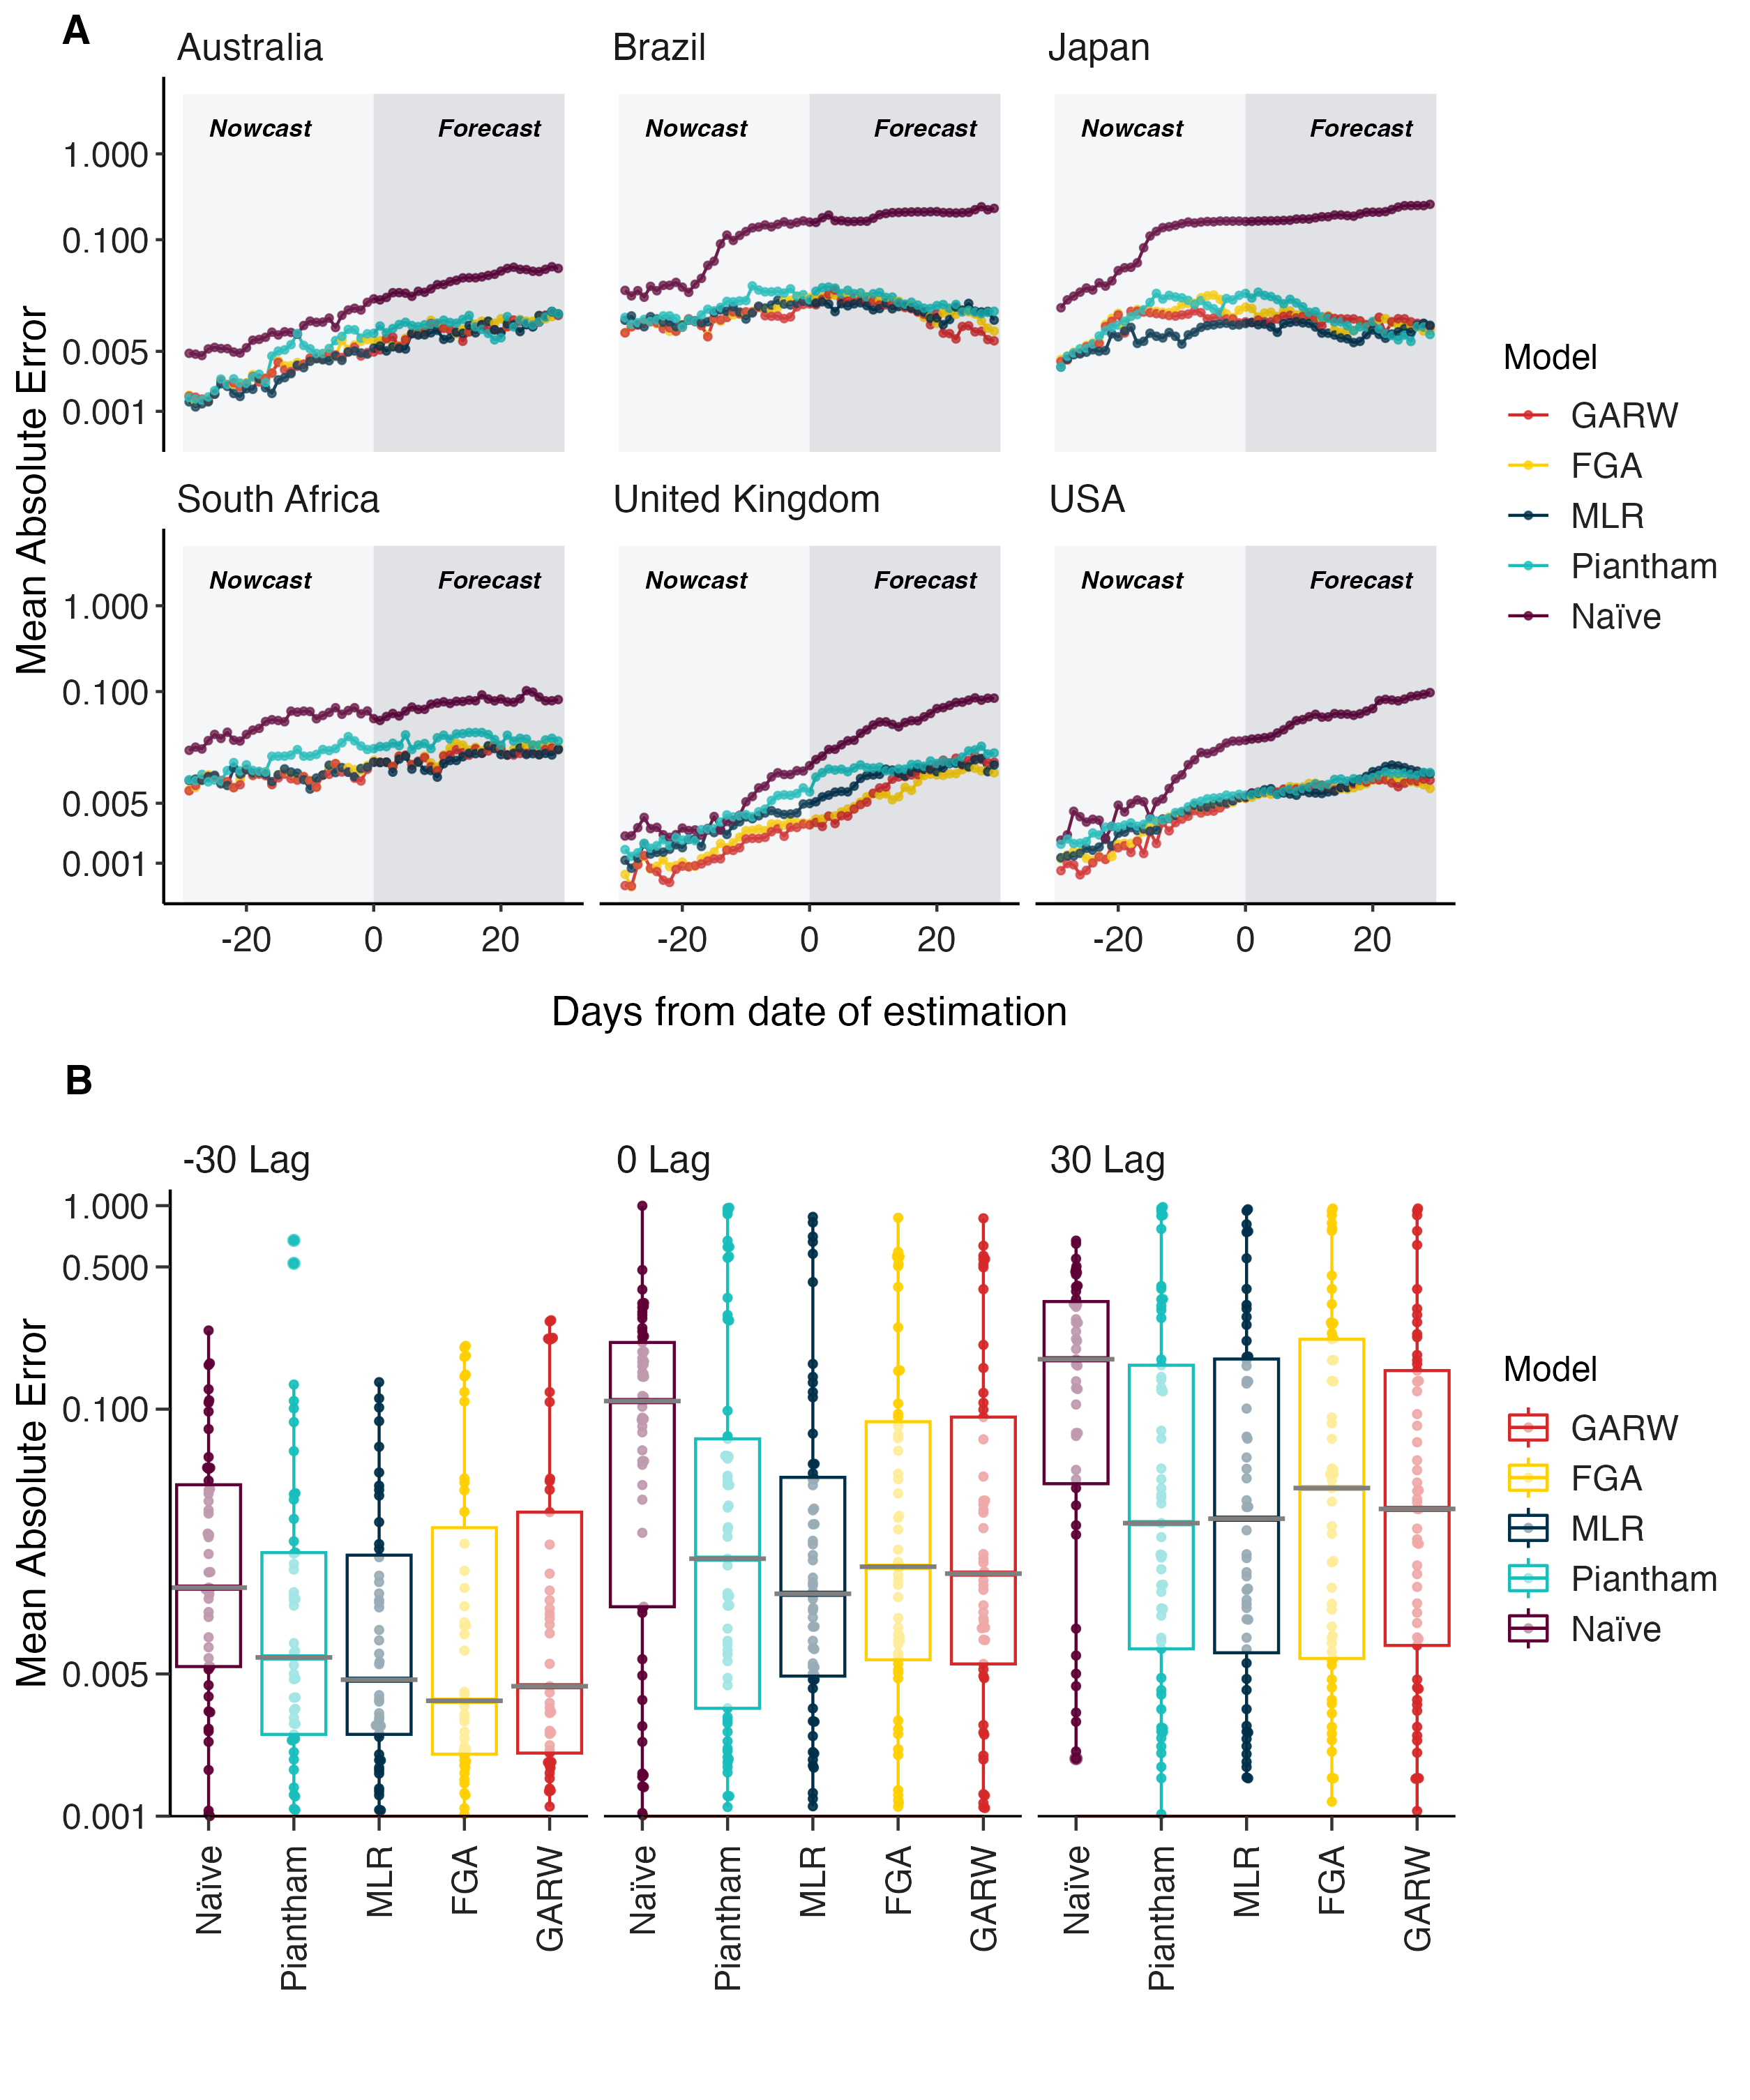
\includegraphics[width=0.8\textwidth]{figures/model_comp.png}
	\caption{\textbf{MAE estimates based on observation date.}
	Figure 2 represents a demonstration of evaluation score (MAE) comparison.
	(A) comparison of progression of error from nowcasting (-30 days) \jhc{Is ``-30 days'' nowcasting or pastcasting?} to forecasting (+30 days) among the five candidate models in six different countries.
	(B) closer look into model performance across all countries for three lag times (-30, 0, 30) showing consistent increase in error with farther lag times.
	}
	\label{fig:model_comp_fig}
\end{figure}


Models were then compared side by side using error quantiles (25,50, and 75th percentile).
The majority of the models evaluated in this study exhibited median error values within the range of 0 to 10 percent of logarithm of mean absolute error (log(MAE)) \jhc{I had trouble wrapping my head around the percent of the log MAE here.} (Figure~\ref{fig:model_comp_fig}A).
Furthermore, we compared the MAE score distribution between models for all countries (Figure~\ref{fig:model_comp_fig}B).
As expected, the results of the analysis show an increase in MAE error for all models as lag or day from estimation increases.

\begin{table}[H]
	\centering
	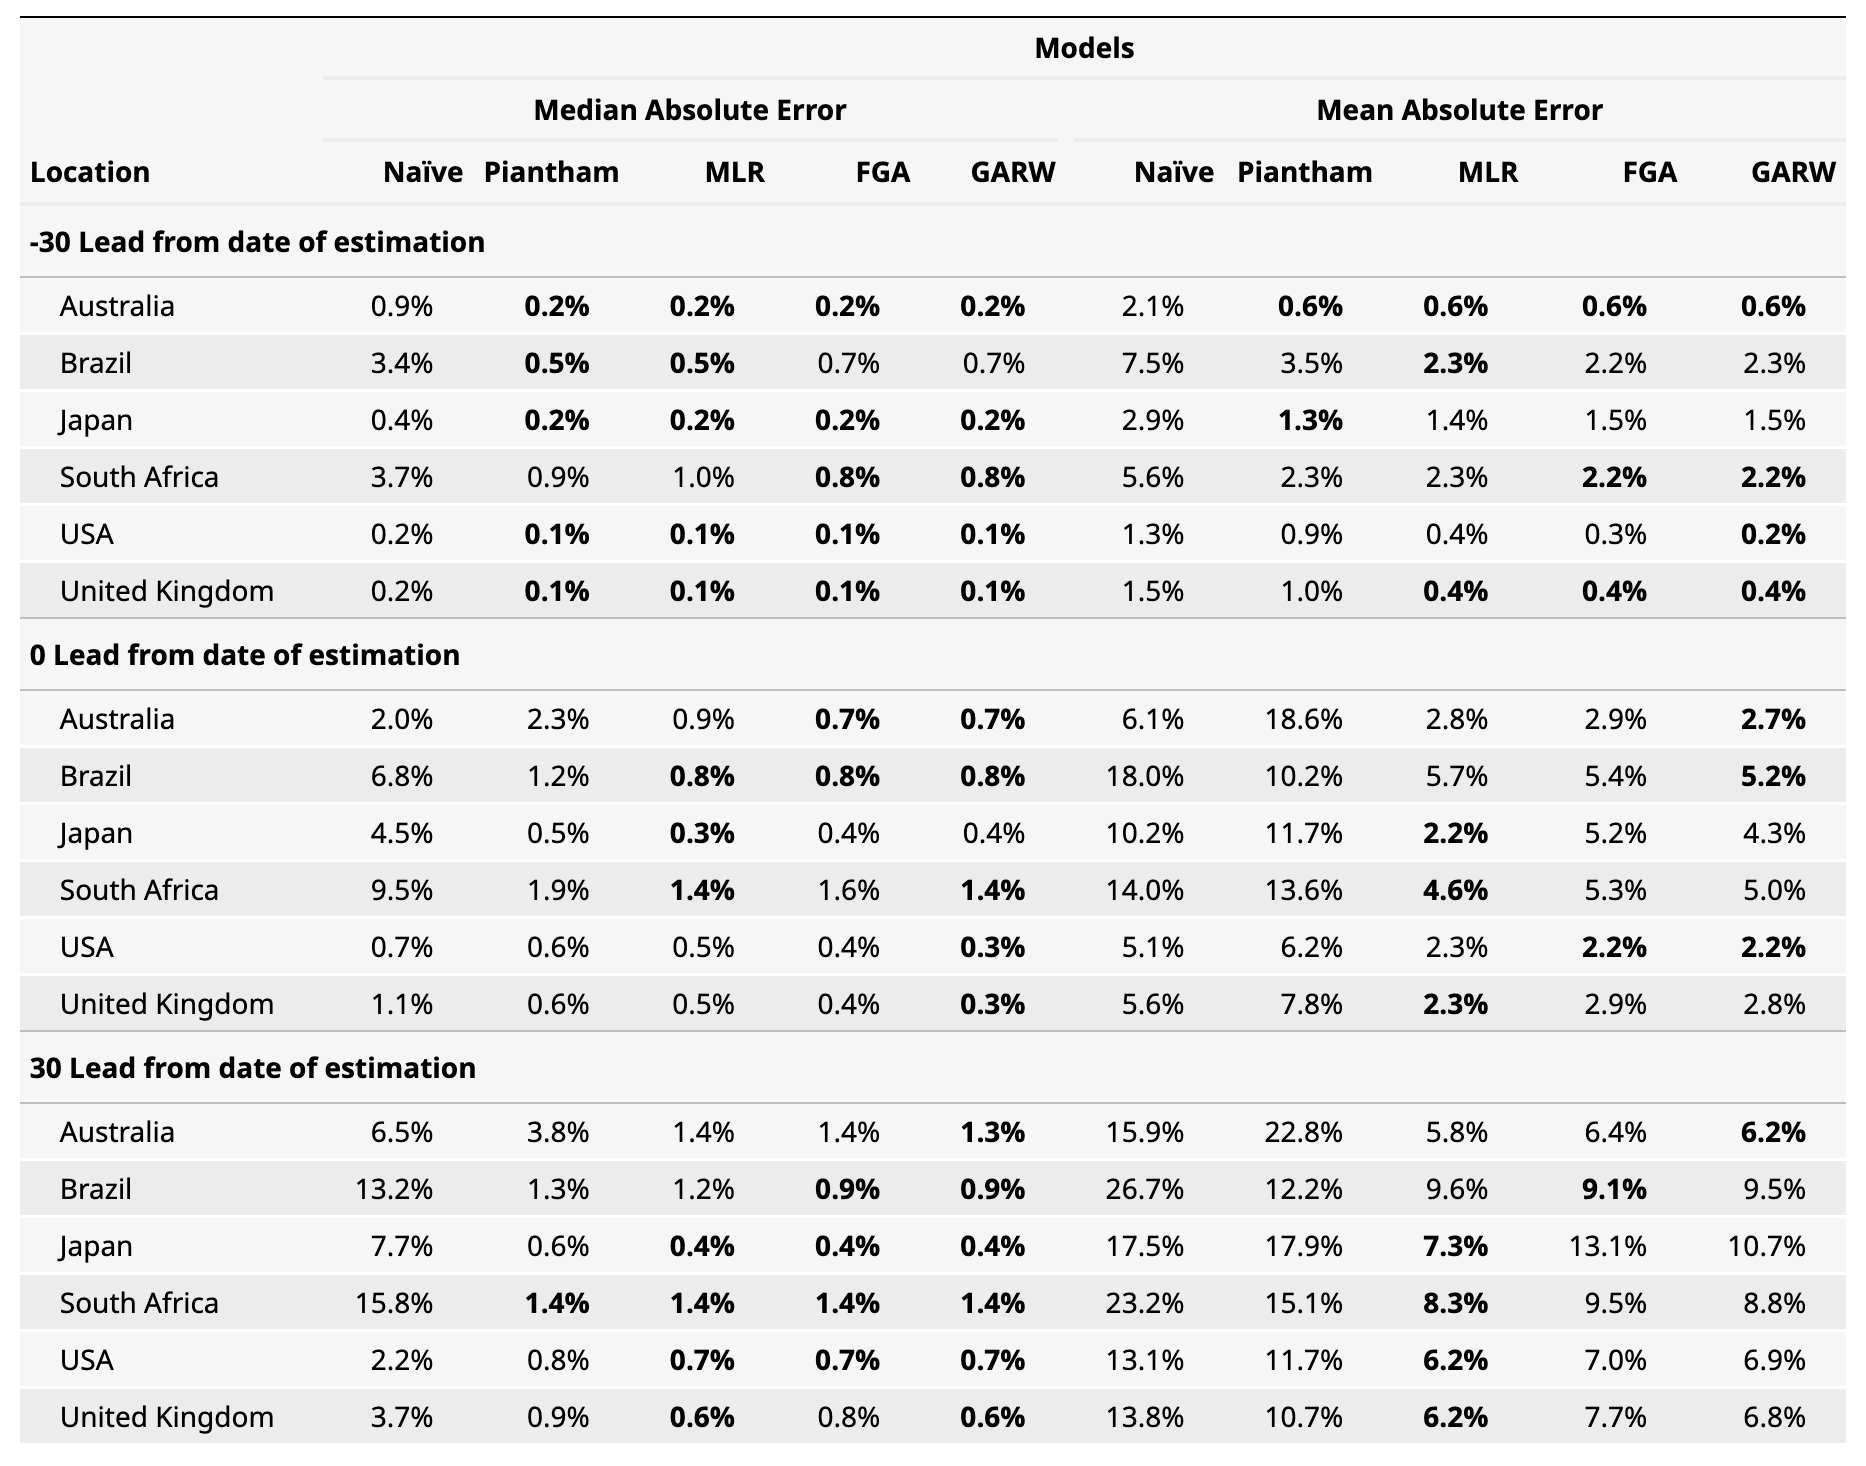
\includegraphics[width=0.6\textwidth]{figures/model_comp_table.png}
	\caption{\textbf{Mean Absolute Error}
	Table 1 demonstrates values of mean absolute error (MAE) for all investigated models at 3 different lag times from the date of estimation (-30, 0, 30).
	Values highlighted exhibit the lowest estimated score allowing for comparisons between models and locations.
    \jhc{Drop the table caption from the PNG figure, since you already have a caption in the text here.}
	}
	\label{table:model_comp_table}
\end{table}

\paragraph{Comparison of Growth Advantages}\ We investigated the behavior of the growth advantage of different variants in the aforementioned countries of interest using the MLR model due to its simplicity and performance.
We standardized the varying growth advantage by estimating the median growth advantage values as of that date.
We observed when and which variants stabilized in each country (Figure~\ref{fig:ga_estimates}).
The majority of countries displayed stabilization with regard to the clades 22A, 22B, and 22C variants, with the exception of Japan.
This discrepancy may be attributed to Japan's limited availability of sequence data and submission delays.
%they mostly stabilized except Japan % and why (motivated us to next step of analysis)

\begin{figure}[H]
	\centering
    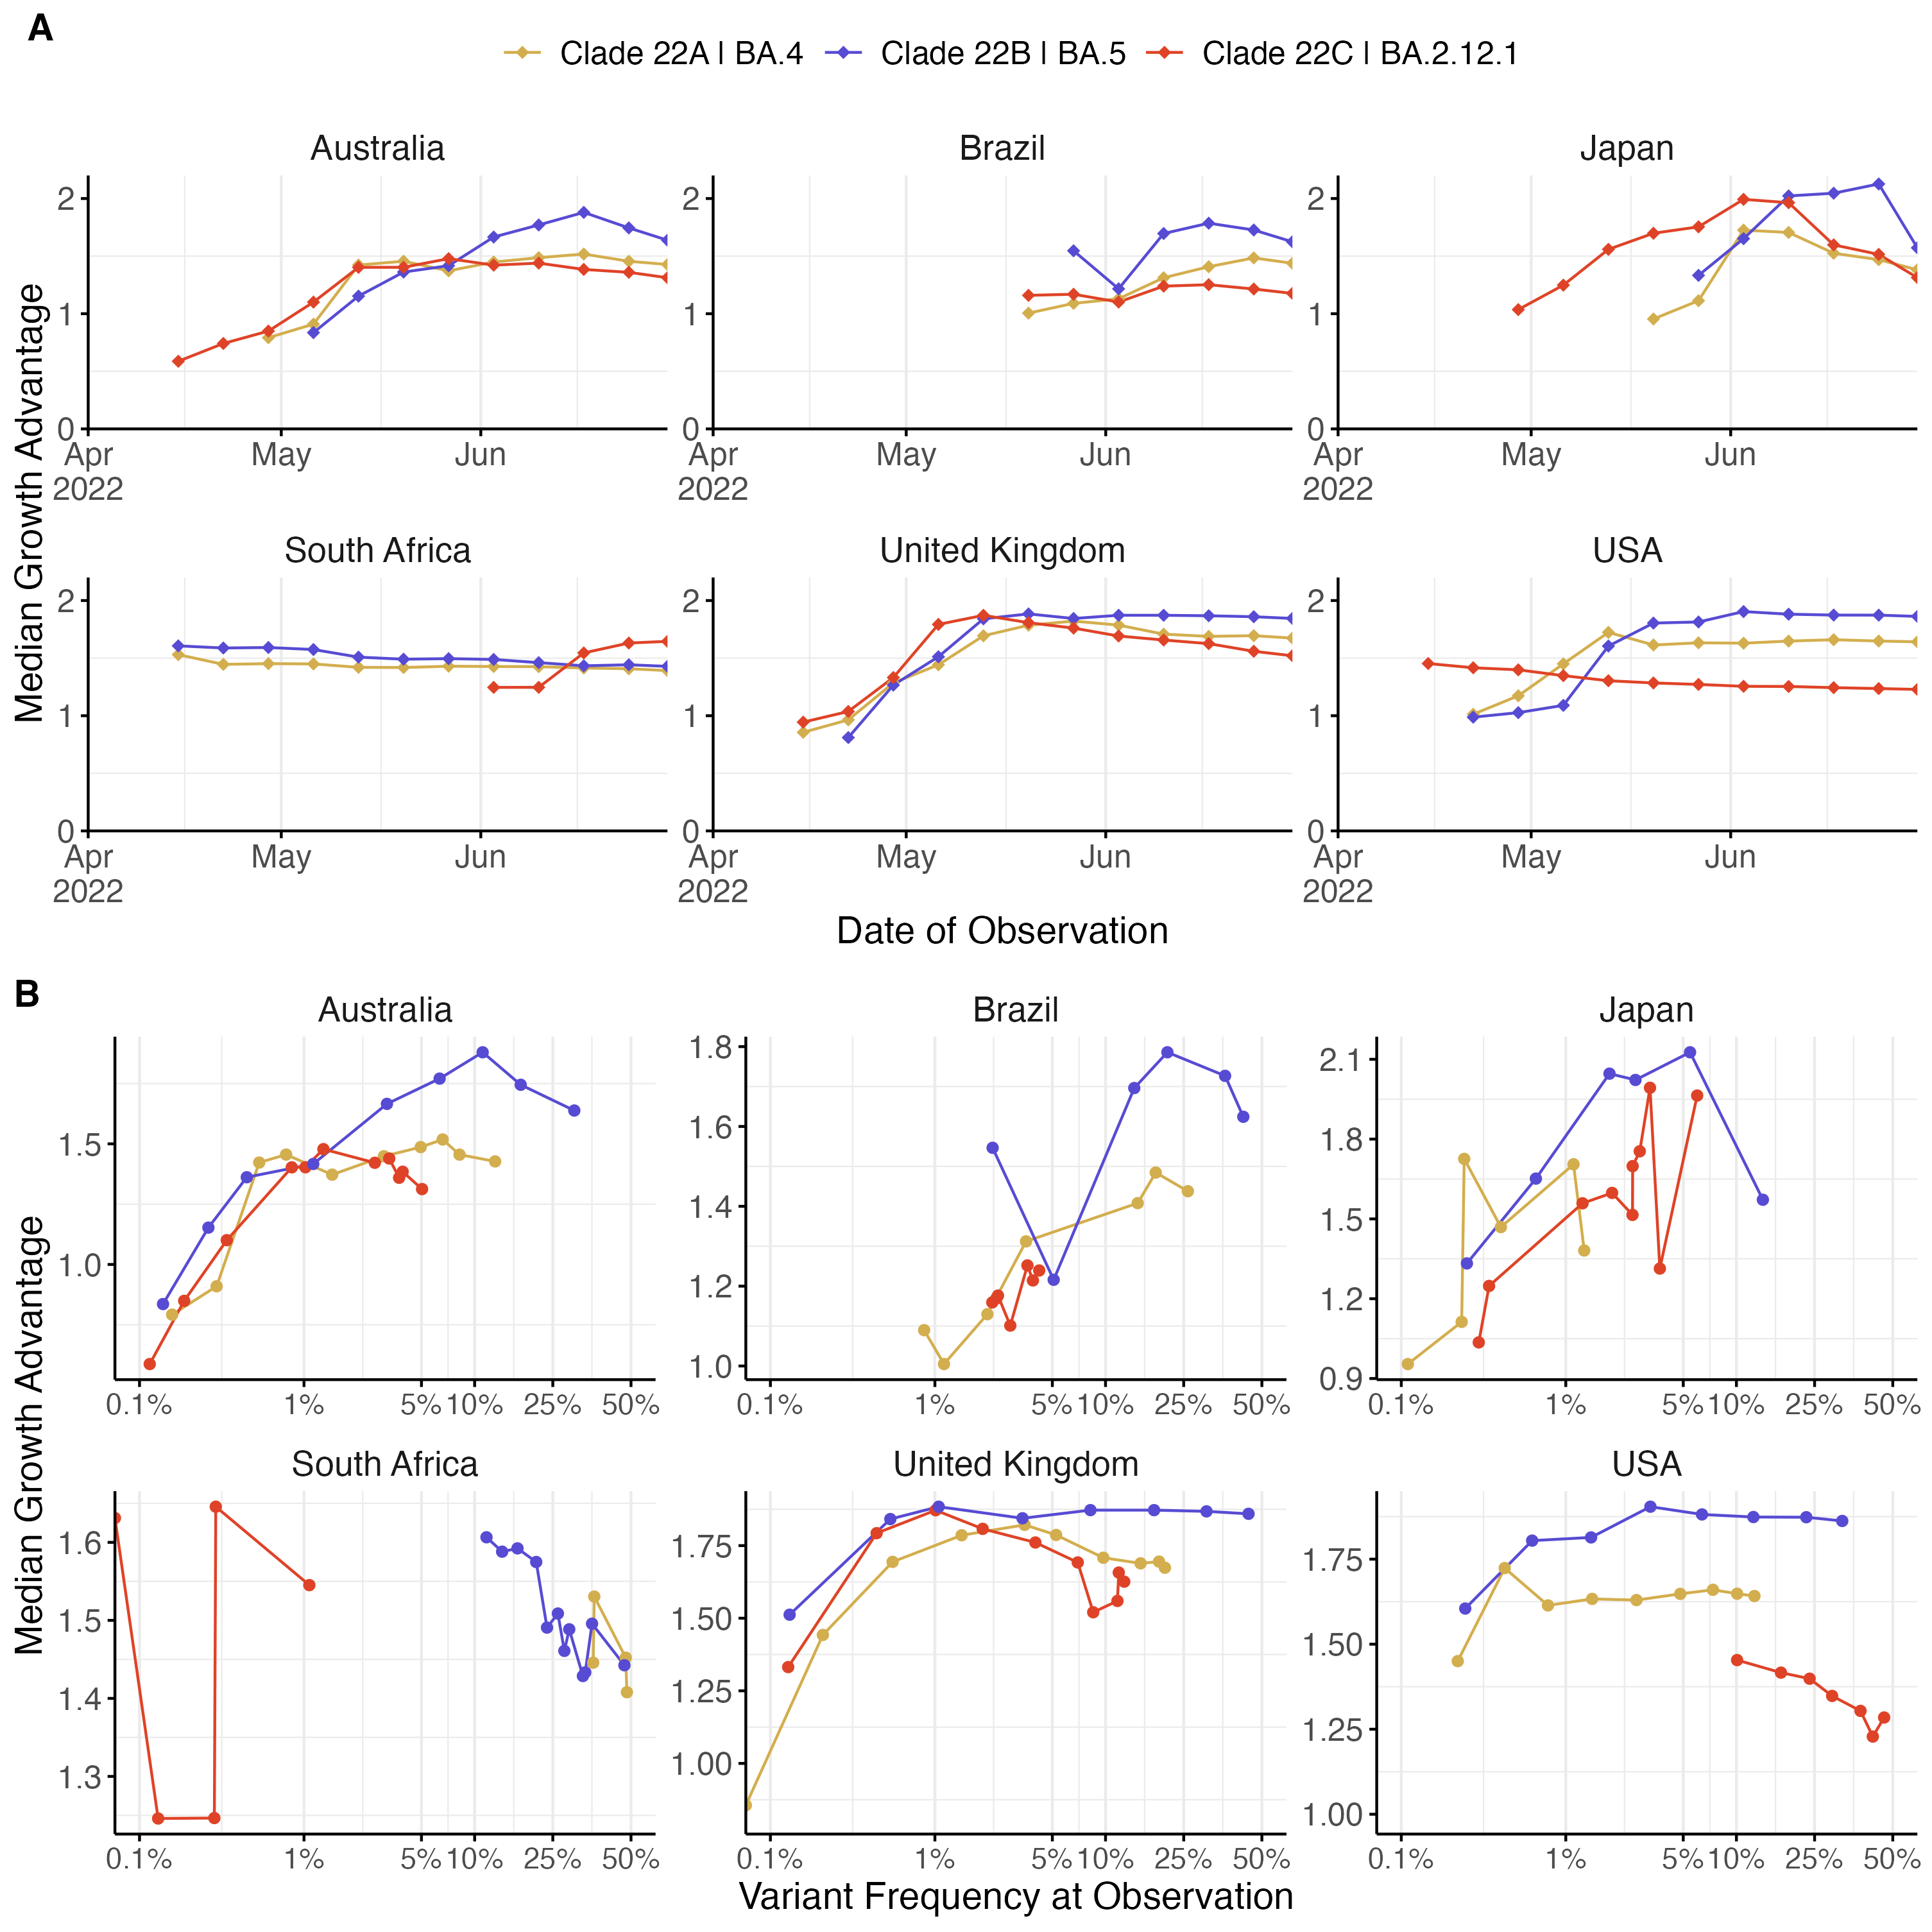
\includegraphics[width=1.1\textwidth]{figures/ga_estimates.png}
	\caption{\textbf{Growth advantage of variants over time}
	Figure 3 demonstrates the stabilization of growth advantage of different clades relative to BA.1 \jhc{This is the first time we see references to Pango lineages which are a third clade nomenclature and not defined elsewhere in the paper.}.
	(A) Differences among growth advantages among three clades in six different countries.
	Noticing how quickly variants dial \jhc{?} and stabilize between different countries \jhc{Fragmented sentence}.
    \jhc{Vertical grid lines don't represent multiples of months or 30 days. Also, Clade 22E in the UK goes off the chart around October.}
	(B) Observation of stabilization of growth advantages according to the percent of variant frequency at observation.
    \jhc{I don't see how panel B shows ``stabilization'' of GAs. Maybe using a shared scale on the y-axis across countries and adding a horizontal line at y=1 would help emphasize convergence to a specific value?}
	}
	\label{fig:ga_estimates}
\end{figure}

\paragraph{Correlates of nowcast error}
\jhc{This section uses present tense, while the prior sections use the past tense.}
We further explore the relationship between variables of interest and the median mean absolute error \jhc{from which model?} across all locations with estimated Spearman correlation.
Variables included are observation dates, median submission delay, fraction of sequences at observation, and sequences available at observation.
We expect that a positive correlation between median submission delay and median MAE such that countries with longer delay exhibit higher errors and a negative correlation between fraction of sequences and sequences available at observation and median MAE such that countries with more robust sequencing efforts show lower errors.
While inter-country variability and other unexplored variables may weaken the correlation, we aimed to uncover meaningful trends into these complex phenomena.
% TODO: Add a sentence summarizing results of the figure
\jhc{Add a sentence or two summarizing results of the figure.}
The results obtained align to initial expectations regarding the trends between the sequencing data and MAE providing insights about the role of sequence submission rate (Figure \ref{fig:vars_of_interest}).


\begin{figure}[H]
	\centering
    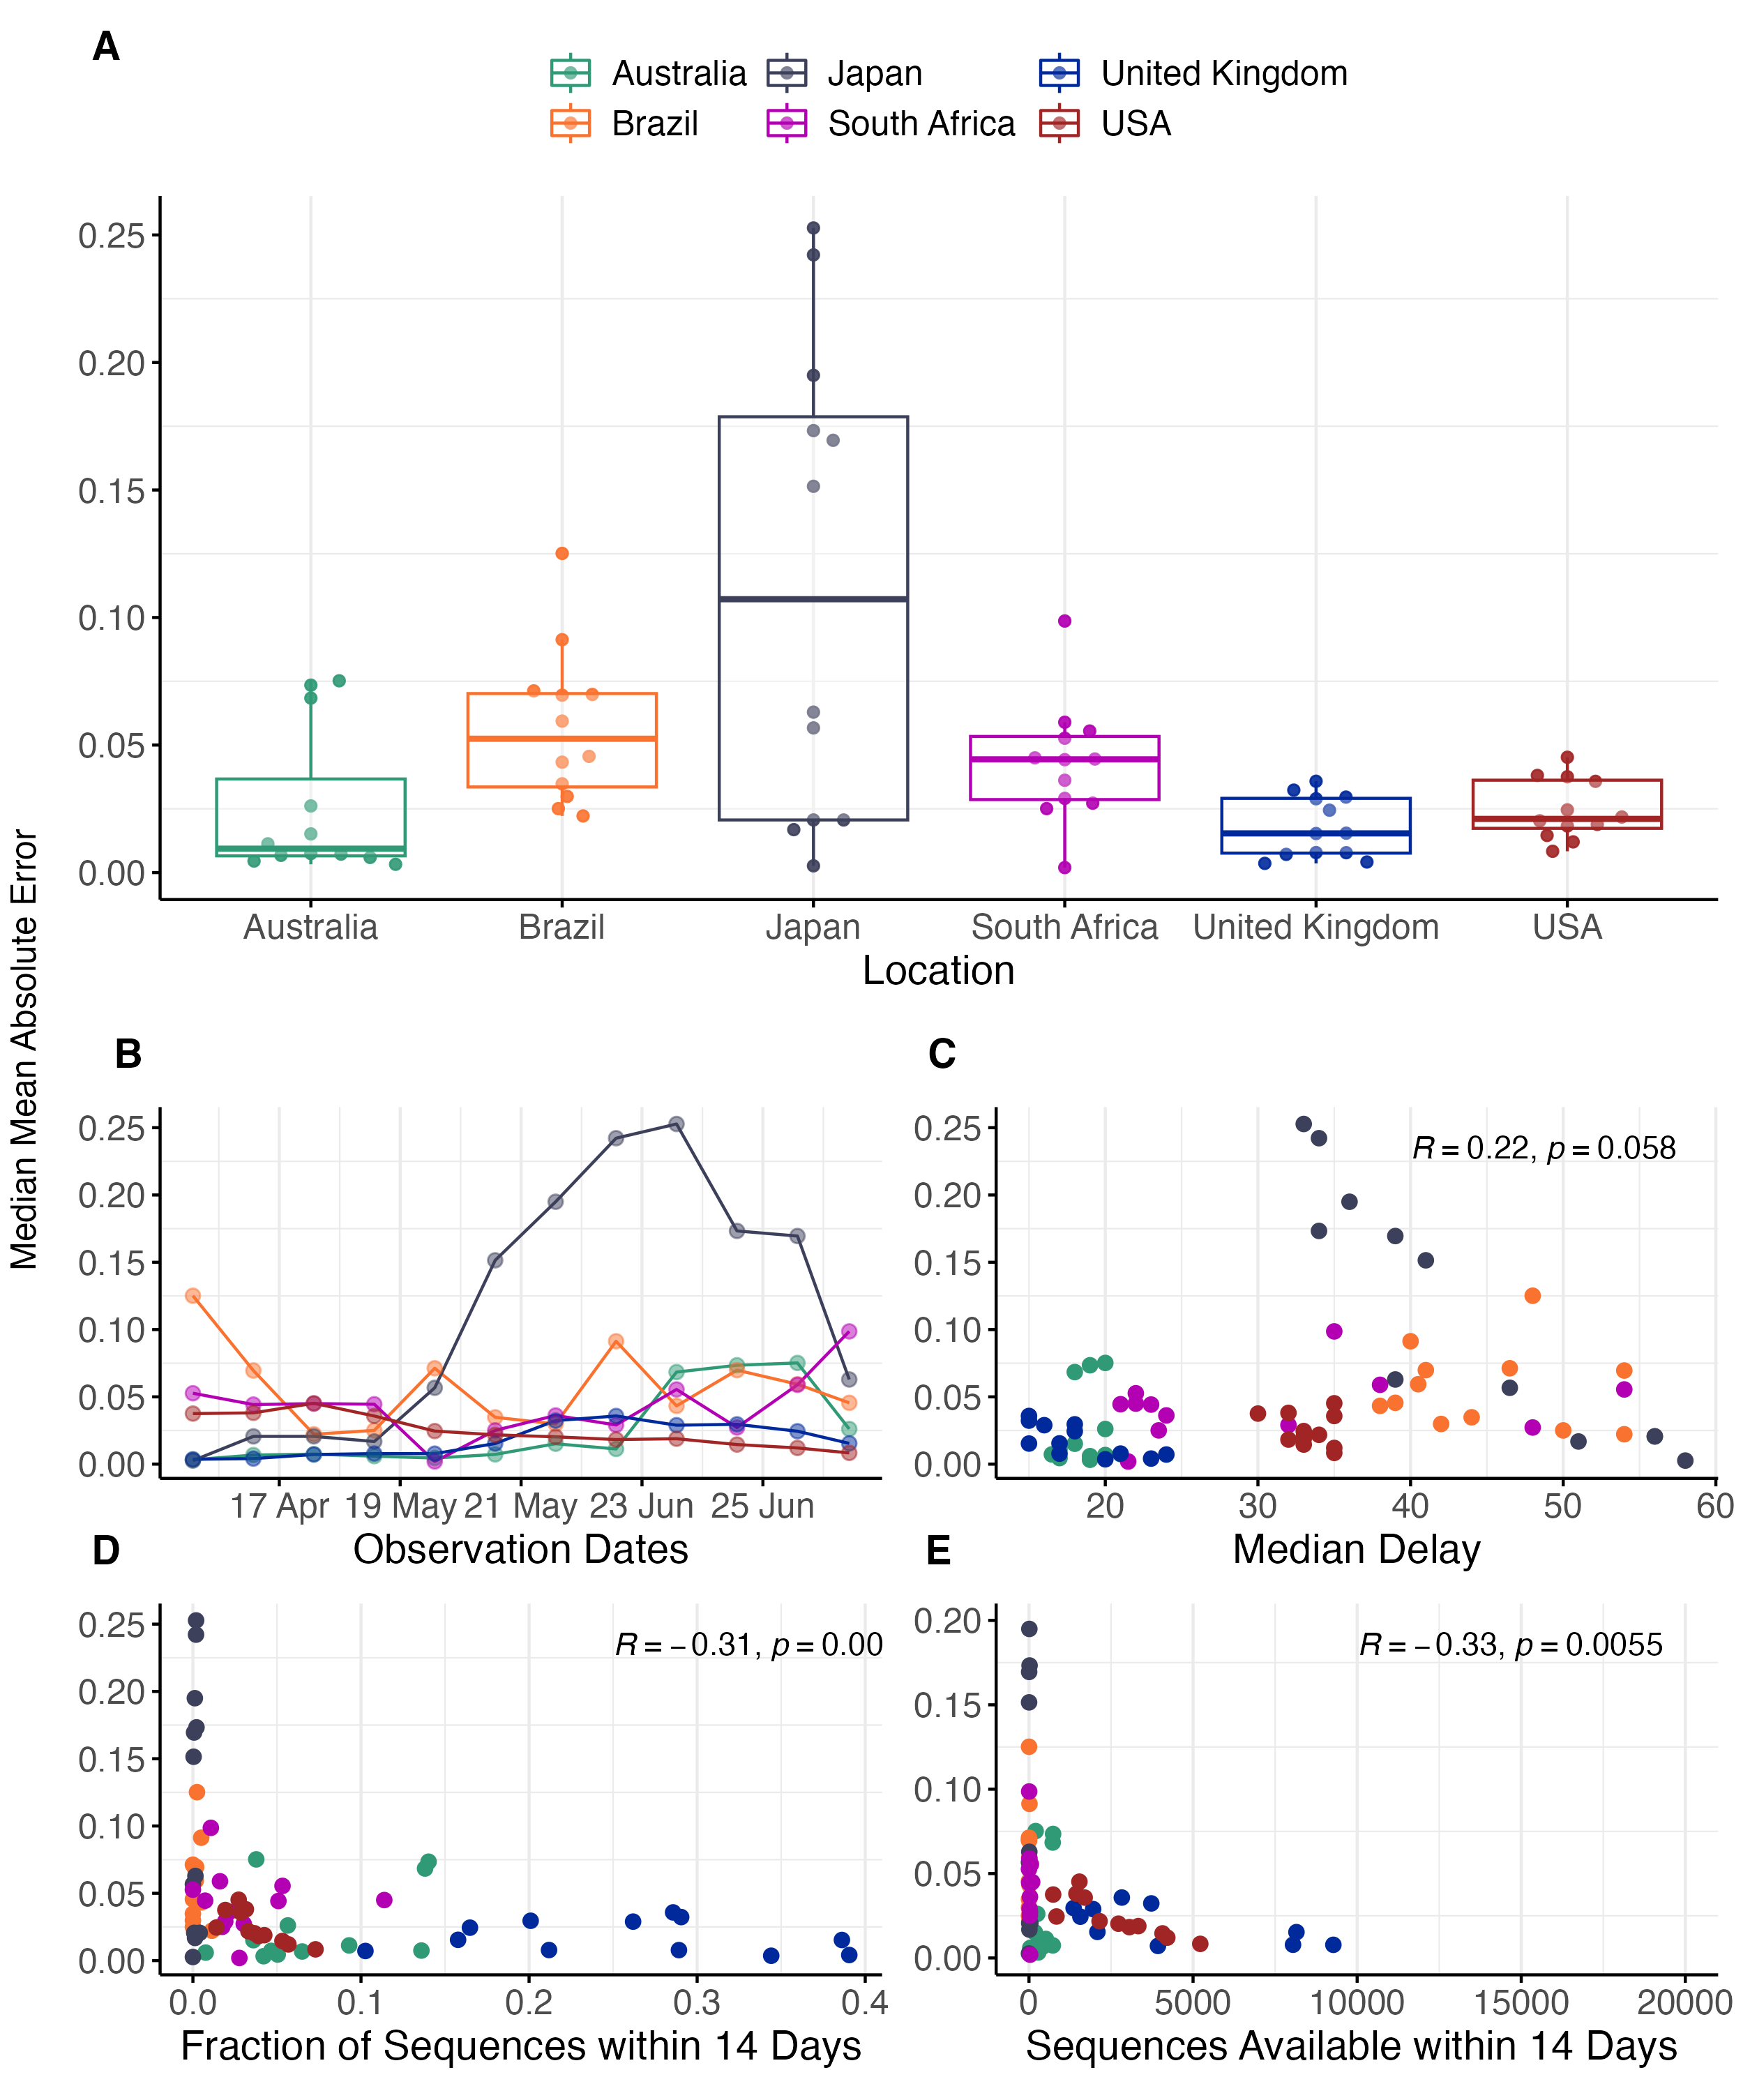
\includegraphics[width=1.1\textwidth]{figures/Var_of_interest.png}
	\caption{\textbf{Variables of interest in predicting forecasting error}
    (A) Forecast MAEs visualized by country. %TODO: Points are medians of ....
    \jhc{What does each point represent?}
    Median MAEs are visualized with observation date (B),
    \jhc{What are the dates on the x axis of panel B? Is ``01'' the day of the month? Why are these x-axis labels different than similar panels in Figures 1 and 3?)}
    median submission delay (C),
    fraction of sequences available at time of observation (D),
    and the total number of sequences available at observation (E).
    For (C-E), we estimate the Spearman correlation between variables of interest and median MAE.
	}
	\label{fig:vars_of_interest}
\end{figure}

\paragraph{Effects of changing sequencing intensity on nowcast error}%

\jhc{This section is also in the present tense. Also, the section heading says ``nowcast error'' but the contents below describe forecasting error.}
We expect that as sequencing intensity decreases, our accuracy in forecasting may vary as we have decreasing levels of resolution in current variant frequencies and estimated growth advantages.
In order to investigate what number of sequences need to collected weekly to keep forecast error within acceptable bounds, we subsample existing sequences from the United Kingdom.
For context, we also compute the weekly sequences collected for selected countries globally (Figure \ref{fig:downscaling}.A).
We select the United Kingdom due to its large counts of available sequences, relatively short submission delay, and low nowcast error (Figure \ref{fig:vars_of_interest}.A,C,E).
We simulate several downscaled data sets by subsampling the collected sequences in the United Kingdom with some \jhc{which?} threshold for number of sequences per week and then fit the MLR model to each of the resulting data sets to see how the forecast accuracy varies with sampling intensity.
From this analysis, we find that increasing the number of sequences per week generally decreases the average error, but there are diminishing returns (Figure \ref{fig:downscaling}).
Additionally, the effect appears to saturate at different values depending on the forecast length.
We find that for 14 and 30 day forecasts sampling at least 1000-2000 sequences per week is appropriate for minimizing forecast error (Figure \ref{fig:downscaling}).


\begin{figure}[H]
    \centering
    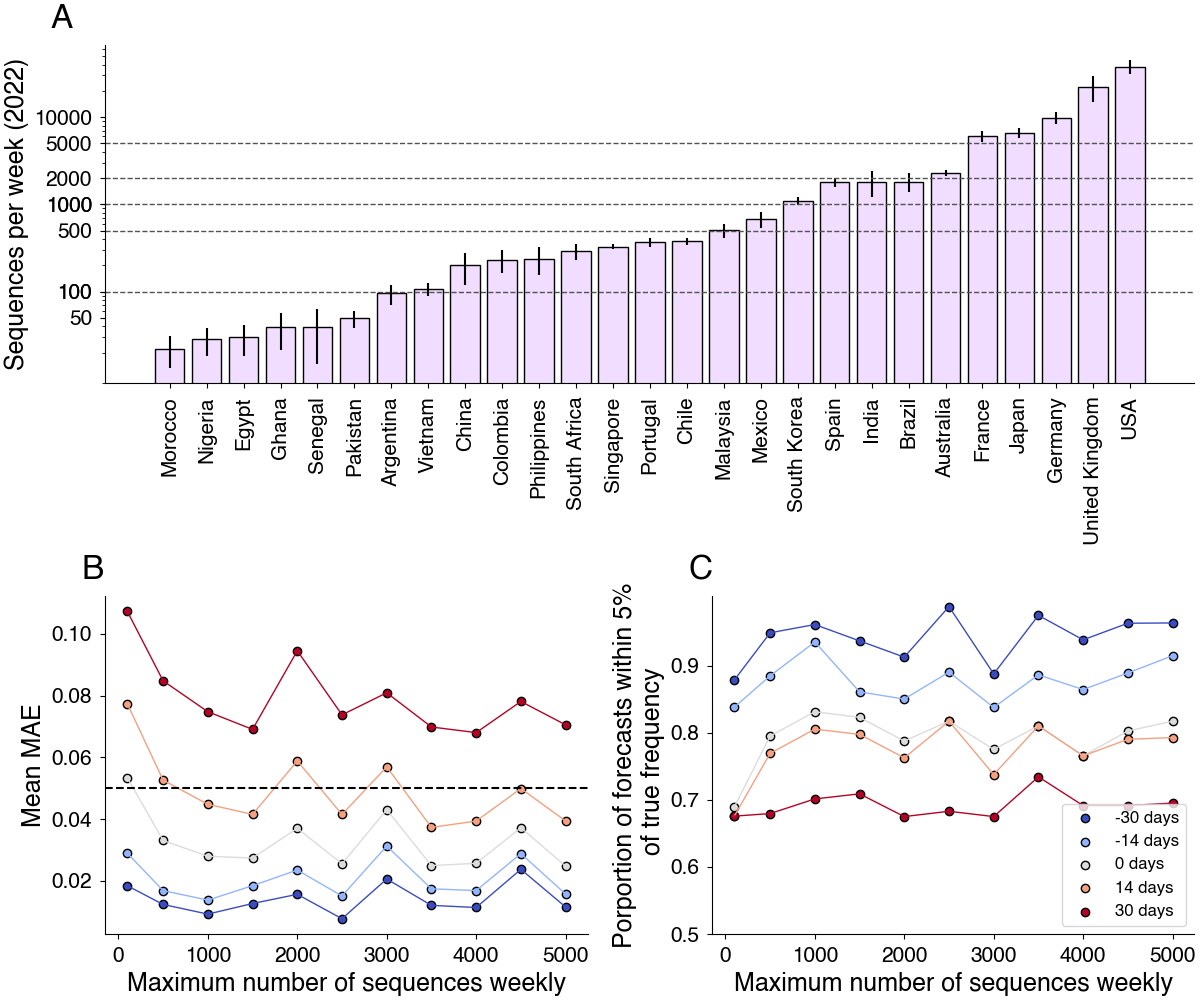
\includegraphics[width=0.8\linewidth]{figures/downscaling_sequencing.png}
    \caption{\textbf{Sequencing intensity affects forecast error.}
    (A) Mean sequences collected per week for selected country. Error bars denote 95\% confidence intervals of the mean. Dashed lines correspond to sampling rates used in (B-E).
    (B, C) Average MAE as a function of sequences collected per week colored by forecast horizon for the United Kingdom and Denmark. Here, ``0 days'' refers to nowcast error and the dash line corresponds to 5\% frequency error.
    (D, E) Proportion of forecasts within 5\% of retrospective frequency as a function of sequences collected for week for the United Kingdom and Denmark.
  }%
    \label{fig:downscaling}
\end{figure}

%%% DISCUSSION %%%
\section*{Discussion}

% Interpretation of the results

%Main findings

%Introducing the discussion

By developing a framework for comparing models of SARS-CoV-2 variant frequency and their forecasts, we find that most models of variant frequency perform well and are able to produce reasonable \jhc{how reasonable?} forecasts.
However, we find that naive models such as a 7-day moving average may not perform well due to the live nature of sequencing efforts e.g. delays between collection and availability of new samples.
Overall, it appears that differences in model accuracy are partially attributable to differences in the surveillance and sequencing efforts.

Consistent with evidence from SARS-CoV-2 time series forecasting analysis \cite{cramer2022unitedforecastinghub}, we find an increase in model errors and their variance as estimates go farther in the future from the observation date.
These long-term forecasts also appear to have heavier tails which indicate increase in extreme values and may be attributable to model break down or the emergence of new variants.

% Through our present framework, we modeled SARS-CoV-2 variant frequencies which allowed us to estimate transmission differences between clades.
% From our initial examination of the data we find that sequencing data exhibit temporal and geographical variation such that data vary based on the date of observation.
% Furthermore, we find that the six countries examined show varying ranges of back-filling of data, submission delays, and missing data.
%
% %patterns of error observed from analysis
% Taking a closer look into the errors generated by our models, we find that there is a consistent patterns of errors (Mean Absolute Error) observed among the different models examined that lend themselves to different interpretation.

%Brazil and japan and south africa? breaking? we wanna see why they break??
%Something may be wrong with them > next analysis?


Our findings suggest that the variations in error patterns observed are likely attributable to the way in which the models handle data issues across different countries.
As such inferences from forecasting models with underlying poor sequencing efforts may not be reliable without a contextual understanding of these limitations.
Additionally, standard modeling practices often involve presenting moving averages of retrospective frequencies of variants as the ``truth''.
However, our analysis of the naive model reveals a substantial discrepancy between the averages of past frequencies and the retrospective truth for all countries, except for the US and UK, where a rigorous sequencing effort is in place.
Importantly, we find that the multinomial logistic regression model (MLR) provides an improvement in accuracy over the naive model for Australia, Brazil, Japan, and South Africa.

%Trevors point about naive model that last 30 days is not actually truth
%Japan: Cornelius > It could be that they have a lot of bunching/overdispersion due to the way labs upload, e.g. one day it’s all North, other day all South etc.

From our analysis of transmission dynamics, we find that it takes a shorter amount of time for different variant clades to stabilize in countries with more robust sequencing efforts.
\jhc{The previous sentence seems to conflate demographics with sequencing capacity.}
Our analysis also suggests that the variability between different countries' growth advantage estimates for different clades may not necessarily be biological but due to data limitations that we show here.
\jhc{What results in the paper support the previous sentence? I don't see where you quantified each country's sequencing capacity and compared that directly to variation in GA.}
We find that at higher frequencies the growth advantage estimates for the clades begin to stabilize though the frequency at which this begins to occur appears to differ by country.
 % To understand why different countries dial in quicker,
%temporal resolution is also important here, why at lower freq US and UK are still doing good

% * these errors affect growth advantage estimates  (figure 3)
% * different variant dynamics happening in different countries which explain why some countries (SA)
% * point about frequency needed for good estimates
% * from investigating variables of interest (which quantify sequencing efforts) we saw that it plays a role in explaining the variation in error

\jhc{Why isn't the following hypothesis the first one to consider instead of sequencing capacity?}
Though our analyses highlight the role of sequencing effort and intensity in reducing forecast error, it is important to note that non-sequencing heterogeneity through the transmission process and pathogen evolution may also explain error.
This could explain why South Africa did not show stabilization in growth advantages due to potentially differing variant dynamics or differences in the sequences effort itself.

We find that there are diminishing returns to increasing sequencing efforts however maintaining consistent sequencing efforts for pathogen surveillance can be done with 1,000-2,000 sequences per week.
\jhc{I see what you're trying to say in the previous sentence, but you might try rephrasing. For example ``maintaining consistent sequencing efforts'' isn't the outcome you get by collecting 1000 sequences; instead you get consistent nowcasting and forecasting estimates.}
This level of sequencing enables robust short-term forecasts of pathogen frequency dynamics at the level of a country and highlights the feasibility of pathogen surveillance for evolutionary forecasting.
Though, we are able to see the overall utility of these methods for providing short-term forecasts, we additionally find that no matter how many sequences are obtained some forecast error is maintained with standard methods for frequency forecasts.


%%% METHODS %%%
\section*{Methods}

\paragraph{Preparing sequence counts and case counts}

\jhc{Methods appear in present tense, but past tense would be appropriate.}
We prepared sequence count datasets to replicate a live nowcasting environment using the Nextstrain-curated SARS-CoV-2 sequence metadata which is created using the GISAID database.
For a given observation date, we filtered to all sequences which were collected 90 days before the observation date.
To properly account for submission delays in this collection process, we additionally filtered to those sequences which were submitted before the observation day.
These sequences are then counted according to their Nextstrain clade to produce sequence counts for each clade each day over the period of interest.
These sequence counts are produced independently for 6 countries including Australia, Brazil, Japan, the United States, the United Kingdom, and South Africa.
We repeated this process for a series of observations days which are the 1st and 15th of each month starting with  Janurary 1st, 2022 and ending with December 15th, 2022 giving a total of 24 datasets for each country.
Since two models (FGA and GARW) also use case counts for their estimates, we additionally prepare data sets using case counts over the time periods of interest as available from Our World in Data.

\paragraph{Frequency dynamics and transmission advantages}%

We implemented and evaluated several models of variant frequencies.
Each of these methods estimate variant frequencies over time and as well as estimate the transmission advantage of given variant relative to a baseline variant $R_{t}^{v} / R_{t}^{u}$.

The 4 models of interest are: Multinomial Logistic Regression (MLR), Piantham model \cite{piantham2021estimating}, a fixed growth advantage model (FGA)  \cite{figgins_bedford_freq_dyn}, and a growth advantage random walk model (GARW)  \cite{figgins_bedford_freq_dyn}.
Details for each of these models can be found in the corresponding citations above.
\jhc{Missing citations for models. Generally, the methods need a bit more description of how the different models work including how they are the same and how they differ.}

We provide a brief mathematical overview of these methods below.

The models mentioned above estimate the frequency  $f_{v}(t)$ of variant $v$ at time $t$ using sequence counts and/or case counts of the form described in the previous section.
All models simultaneously estimate the variant transmission advantages $\Delta_{v} = \frac{R_{t}^{v}}{R_{t}^{\text{pivot}}}$ where $R_{t}^{v}$ is the effective reproduction number for variant $v$.
We can interpret these transmission advantages as the relative effective reproduction number of a variant relative to some reference variant.

The multinomial logistic regression model estimates a fixed growth advantage using logistic regression with a variant-specific intercept and time coefficient, so that the frequency of variant $v$ at time $t$ can be modeled as
\begin{align*}
    f_{v}(t) = \frac{\exp(\alpha_{v} + \delta_{v} t)}{\sum_{u} \exp(\alpha_{u} + \delta_{u} t)},
\end{align*}
where $\Delta_{v} = \exp(\delta_{v} \tau)$ for some fixed generation time $\tau$.
The Piantham model relies on an approximation to the renewal equation wherein new infections do not vary greatly over the generation time of the virus.
This model generalizes the MLR in that it accounts for non-fixed generation time though it assumes little overall case growth. \cite{piantham2021estimating}

The fixed growth advantage model uses a renewal equation model based on both case counts and sequence counts, but assumes that the growth advantage $\Delta_{v}$ is constant in time. \cite{figgins_bedford_freq_dyn}
The growth advantage random walk model also uses a renewal equation model based on both case counts and sequences, but allows variant growth advantages to vary smoothly in time. \cite{figgins_bedford_freq_dyn}

The models used all differ in the complexity of their assumptions in computing the variant growth advantage which may affect forecasting accuracy.
Growth advantages presented in this manuscript are estimated relative to the baseline Omicron 21L (BA.1) strain, providing a point of reference for competing growth advantages and how median values change over time.
Further details on the model formats can be found in their respective citations.
All models were implemented using the evofr (evolutionary forecasting) software package in Python (https://pypi.org/project/evofr/) using Numpyro for inference.

We compare the four models to a naive model which is implemented as a 7-day moving average on the retrospective raw frequencies.

\paragraph{Evaluation Criteria}

We evaluate the error between the model predicted frequencies and the truth set averaged across each variant at a given time point using the mean absolute error (MAE).

\paragraph{Generating predictors of error}

We explored four key variables to describe the effect of sequencing efforts on nowcast errors and found their Spearman correlations with the nowcast errors.
These variables are defined as fraction of sequences available within 14 days of the prediction time, total sequences availability within 14 days of the prediction time, median delay of sequence submission, and lag time from prediction day subsequently for each location (Figure~\ref{fig:vars_of_interest}).
To calculate these variables, we selected a 14-day window of data before each and every observation date and used the collection and submission dates to determine their availability in addition to the period of discrepancy between the collection and submission for each country.
All variables were calculated using Rstudio statistical software \jhc{Cite RStudio.}.

%TODO: Add details on how we generate points for \ref{fig:vars_of_interest}


\paragraph{Downscaling historical sequencing effort}

We explored the effects of scaling back sequencing efforts to assess the effect of sequencing volume on nowcast and forecast errors.
Using sequences from the United Kingdom, we subsampled existing sequences at a rate of 100, 500, 1000, 1500, 2000, 2500, 3000, 3500, 4000, 4500, 5000 sequences per week at various \jhc{which?} observation dates throughout the pandemic.
We then fit the MLR forecast model to each resulting data set and forecast up to 30 days after observation date.
We then compared these forecasts to the truth set in previous sections to compute the forecast error for each model.

To better understand how the forecast error varies with sequencing intensity and forecast length, we computed the fraction of forecasts within a certain ``acceptable'' \jhc{maybe drop ``acceptable'' here, since the 5\% threshold is arbitrary.} error tolerance (5\% MAE) as well as the average error at difference sequence threshold and lag times.


\section*{Data and code accessibility}

Sequence data including date and location of collection as well as clade annotation was obtained via the Nextstrain-curated
dataset that pulls data from GISAID database \jhc{Create a GISAID DOI or acknowledgements table for all of the distinct sequences you used in this analysis. They provide a tool now to simplify the DOI creation.}.


Derived data of sequence counts and case counts, along with all source code used to analyze
this data and produce figures is available via the GitHub repository https://github.com/blab/ncov-forecasting-fit


%%% REFERENCES %%%
\bibliographystyle{plos}
\bibliography{ncov-forecasting-fit.bib}

\end{document}
